\chapter{Evaluation}
\label{ch:evaluation}

\section{Evaluation Methodology}
\label{sec:eval_methodology}

This chapter evaluates the pipeline against the four success criteria
committed in Chapter~\ref{ch:introduction}: detector mAP@50 $\geq 0.80$,
tracking HOTA $\geq 0.45$, team-assignment F1 $\geq 0.85$, and
qualitatively coherent tactical outputs. Each criterion is addressed by
the section that owns the corresponding pipeline stage, with verdicts
issued explicitly where the available evidence permits one.

The evaluation operates at three levels of evidence, chosen to match
the type of claim being made. \emph{Component-level} evaluation
(Sections~\ref{sec:eval_detection} and~\ref{sec:eval_pitch}) uses the
held-out test splits of the three training datasets and reports the
standard object-detection and pose metrics defined in
Sections~\ref{subsec:background_iou_nms}
and~\ref{subsec:background_tracking_metrics}: precision, recall, mAP at
IoU thresholds 0.50 and 0.50:0.95, per-class breakdowns, and confusion
matrices. These metrics are directly comparable to the
broadcast-football literature
\cite{Cioppa2022,Theiner2022,Magera2025}.
\emph{Integration-level} evaluation
(Sections~\ref{sec:eval_tracking} and~\ref{sec:eval_team})
characterises stages whose behaviour depends on temporal context —
tracking continuity, team-label stability — and therefore cannot be
assessed on still images. Tracking is evaluated on a combined
evaluation set comprising five SportsMOT-football validation
sequences~\cite{Cui2023SportsMOT} and one hand-labelled broadcast clip
of $750$~frames annotated in MOTChallenge format, with HOTA, MOTA, IDF1,
and identity-switch counts computed via TrackEval. Team classification
is evaluated on three independent broadcast clips with manually
labelled torso crops, under both an upper-bound full-crop clustering
regime and a deployment-realistic warm-up split.
\emph{System-level} evaluation
(Sections~\ref{sec:eval_tactical} and~\ref{sec:eval_runtime}) examines
the end-to-end outputs — pass and offside event logs, per-player
statistics, heatmaps, runtime — on full pipeline runs against the same
three broadcast clips, with event ground truth obtained by visual
inspection of the annotated outputs.

The evaluation is scoped by the failure-handling table established in
Section~\ref{sec:methodology_failure_handling}: claims are made only
within the operational regime that table defines, and degraded-input
behaviour is characterised in Section~\ref{sec:eval_failures} rather
than being treated as out-of-scope. Where a metric or comparison is
omitted, the omission is stated and justified rather than silently
dropped.

\section{Detection Performance}
\label{sec:eval_detection}

The two trained detectors are evaluated on the held-out test splits of
their respective datasets (75 images / 1{,}875 instances for the generic
detector; 119 images / 119 instances for the ball detector) using the
standard COCO-style protocol described in
Section~\ref{subsec:background_iou_nms}. Results were obtained with the
weights selected by validation \texttt{mAP@50:95} (epoch 40 for the
generic detector, epoch 143 for the ball detector). All metrics are
reported on the test split only; validation figures are tabulated in
the methodology training reports and are not duplicated here.

\subsection{Generic four-class detector}

Table~\ref{tab:detector_per_class} presents the per-class test metrics.
The generic detector achieves a mean test \texttt{mAP@50} of
$0.855$, exceeding the success criterion (i) target of $0.80$
(Chapter~\ref{ch:introduction}). The aggregate figure, however, masks a
sharply bimodal per-class distribution: Player, Goalkeeper, and Referee
are all near-saturated ($\text{mAP@50} \geq 0.98$, $\text{F1} \geq 0.96$),
whereas the Ball class achieves $\text{mAP@50} = 0.459$ at recall $0.39$
under the per-class summary protocol.
Figure~\ref{fig:generic_pr} shows the corresponding precision--recall
curves: the three person classes track the upper envelope of the plot
while the Ball curve collapses below recall $0.8$, isolating the
small-object localisation problem from the rest of the detection task.

\begin{table}[h]
\centering
\small
\begin{tabular}{lrrrrr}
\toprule
Class & P & R & F1 & mAP@50 & mAP@50:95 \\
\midrule
Ball       & 0.818 & 0.393 & 0.531 & 0.459 & 0.194 \\
Goalkeeper & 0.953 & 0.983 & 0.968 & 0.982 & 0.808 \\
Player     & 0.991 & 0.991 & 0.991 & 0.995 & 0.823 \\
Referee    & 0.939 & 0.981 & 0.960 & 0.983 & 0.707 \\
\midrule
Mean       & 0.925 & 0.837 & 0.873 & 0.855 & 0.633 \\
\bottomrule
\end{tabular}
\caption[Generic detector: per-class test performance.]{Generic
detector test-set performance. Player, Goalkeeper, and Referee classes
are near-saturated; the Ball class limits aggregate
\texttt{mAP@50:95}.}
\label{tab:detector_per_class}
\end{table}

\begin{figure}[h]
\centering
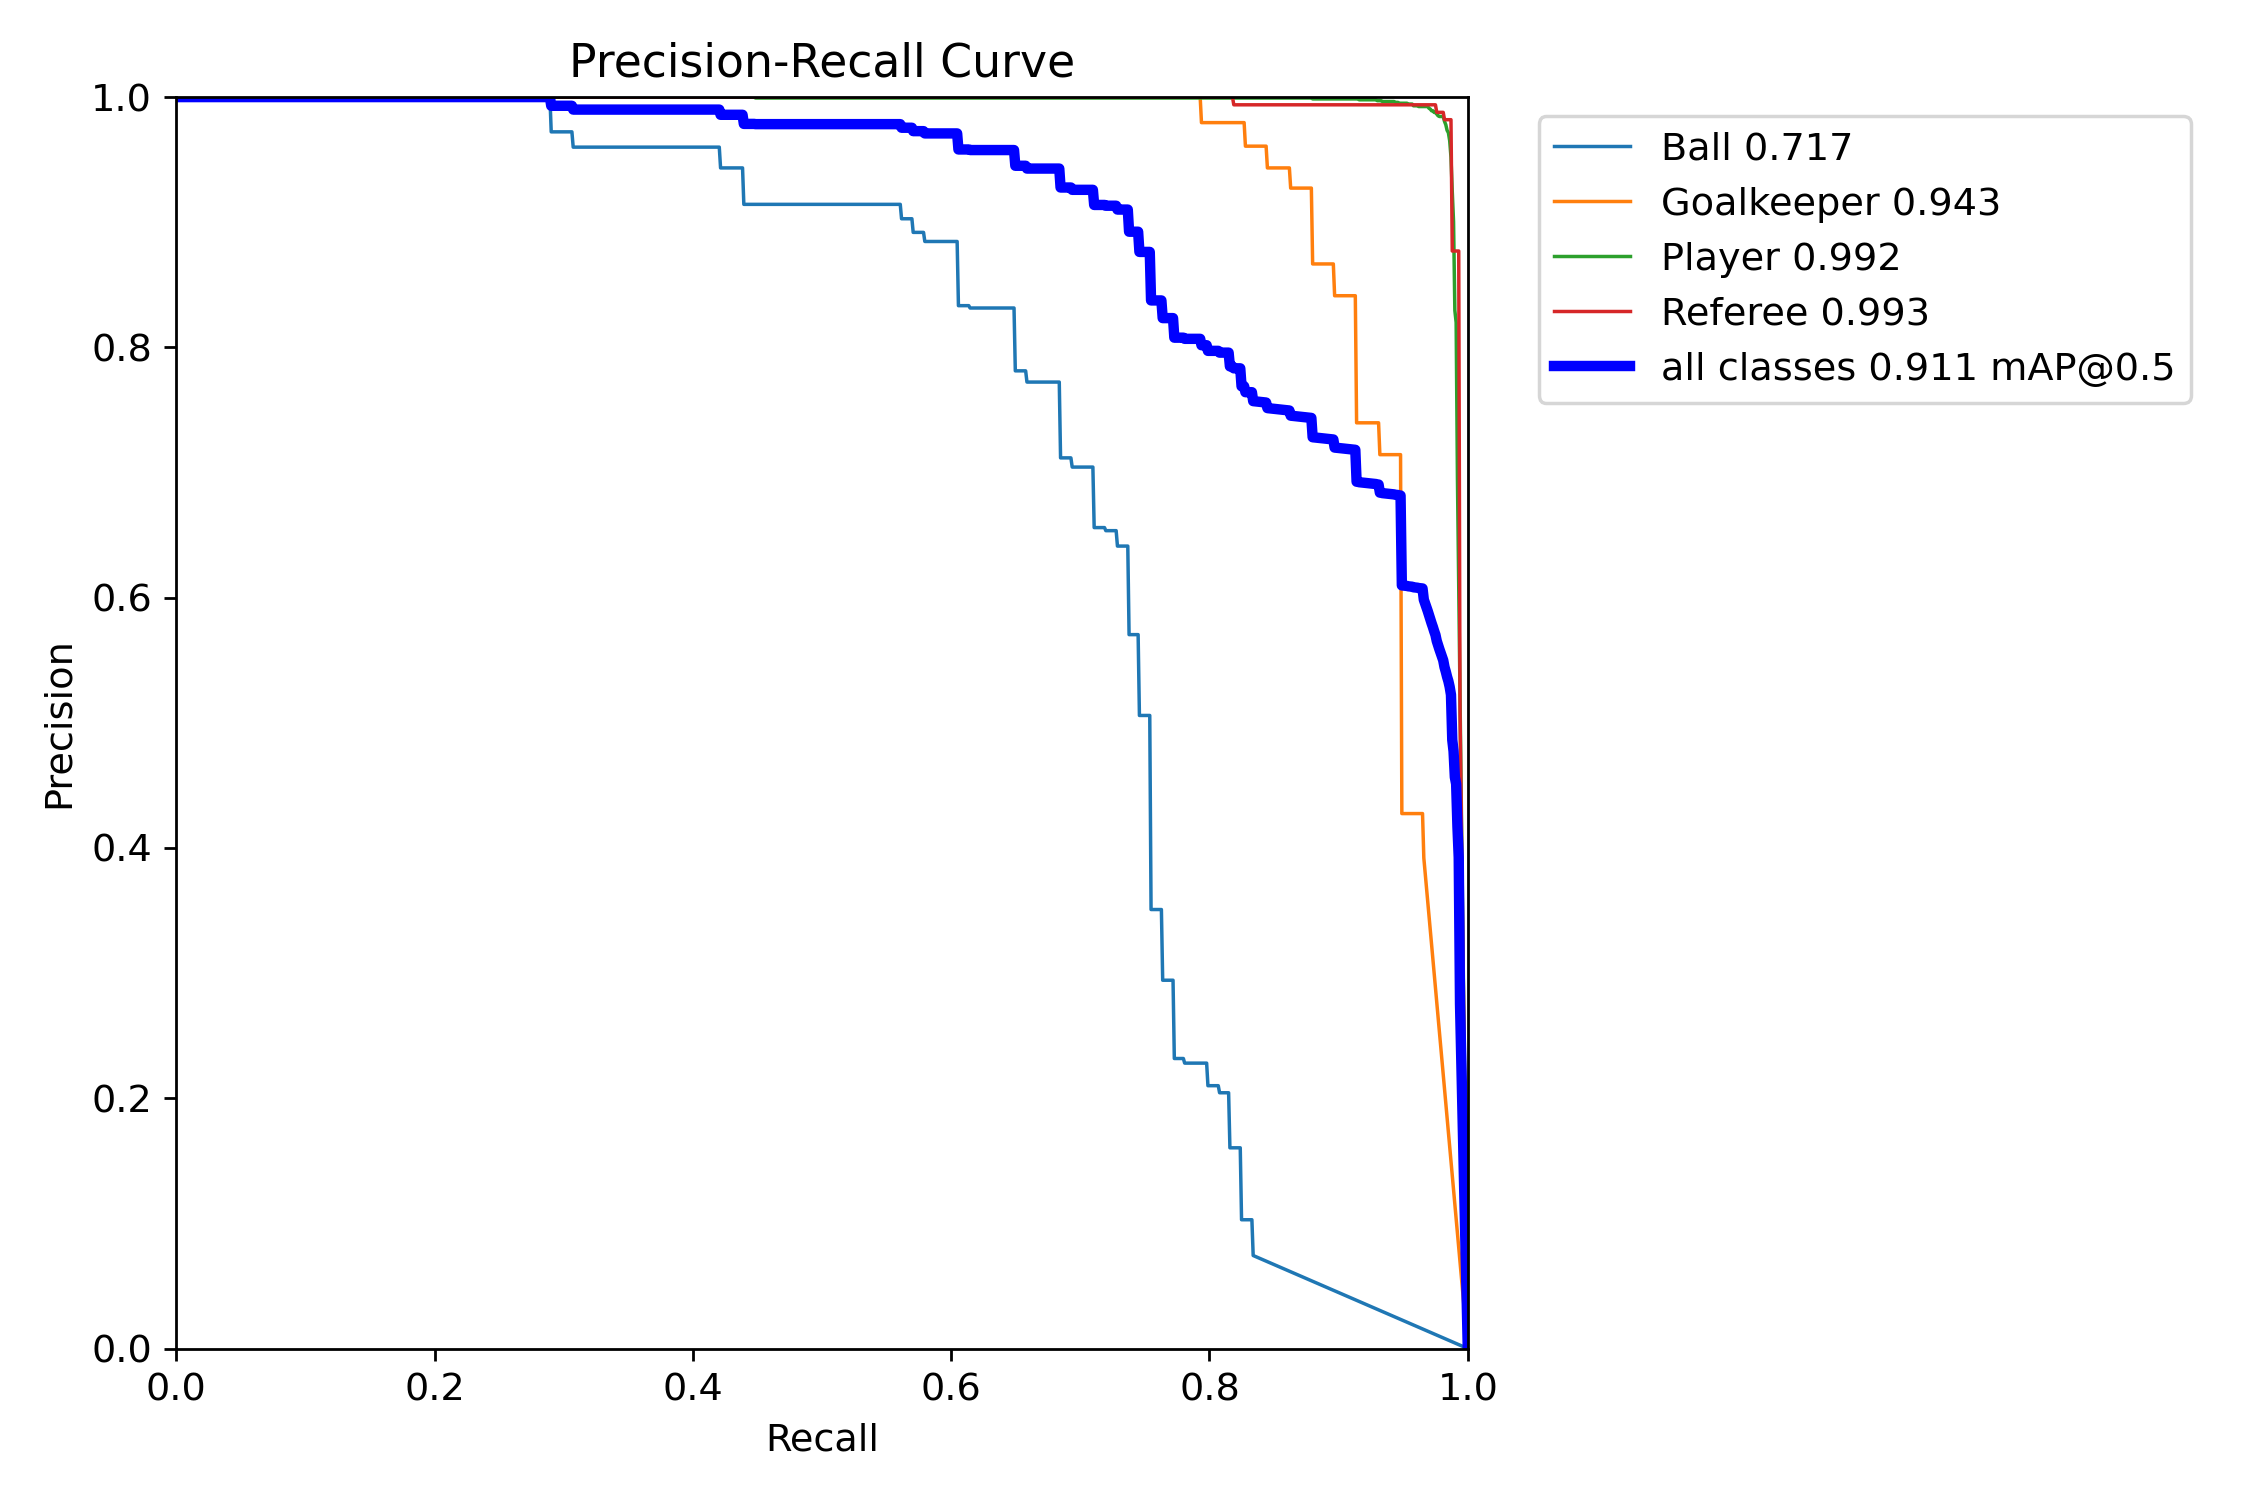
\includegraphics[width=0.7\textwidth]{images/04-evaluation/generic_pr.png}
\caption[Generic detector: precision--recall curves.]{Precision--recall
curves for the generic four-class detector on the test split. The
three person classes (Player, Referee, Goalkeeper) sit on the upper
envelope of the plot, while the Ball class collapses sharply once
recall exceeds $0.75$, accounting for the bulk of the gap between
mean \texttt{mAP@50} and the person-class scores.}
\label{fig:generic_pr}
\end{figure}

The normalised test confusion matrix
(Figure~\ref{fig:generic_cm_norm}) localises the failure modes. Of
true balls, $31\%$ are confused with background, and of background
predictions, $40\%$ are predicted as ball. This indicates that the
small target size and low contrast against pitch grain are the
dominant nuisance for ball detection at $1280\times1280$, consistent
with \cite{Cioppa2022}. A second mode is the $10.3\%$
Goalkeeper-as-Player confusion ($6/58$ test instances), driven by the
$21\!:\!1$ training imbalance ($12{,}311$ Player versus $465$
Goalkeeper instances) and by appearance overlap when goalkeepers play
upfield. This confusion motivates the image-space goalkeeper resolver
of Section~\ref{subsec:methodology_gk_resolver}, evaluated separately
in Section~\ref{sec:eval_team}.

\begin{figure}[h]
\centering
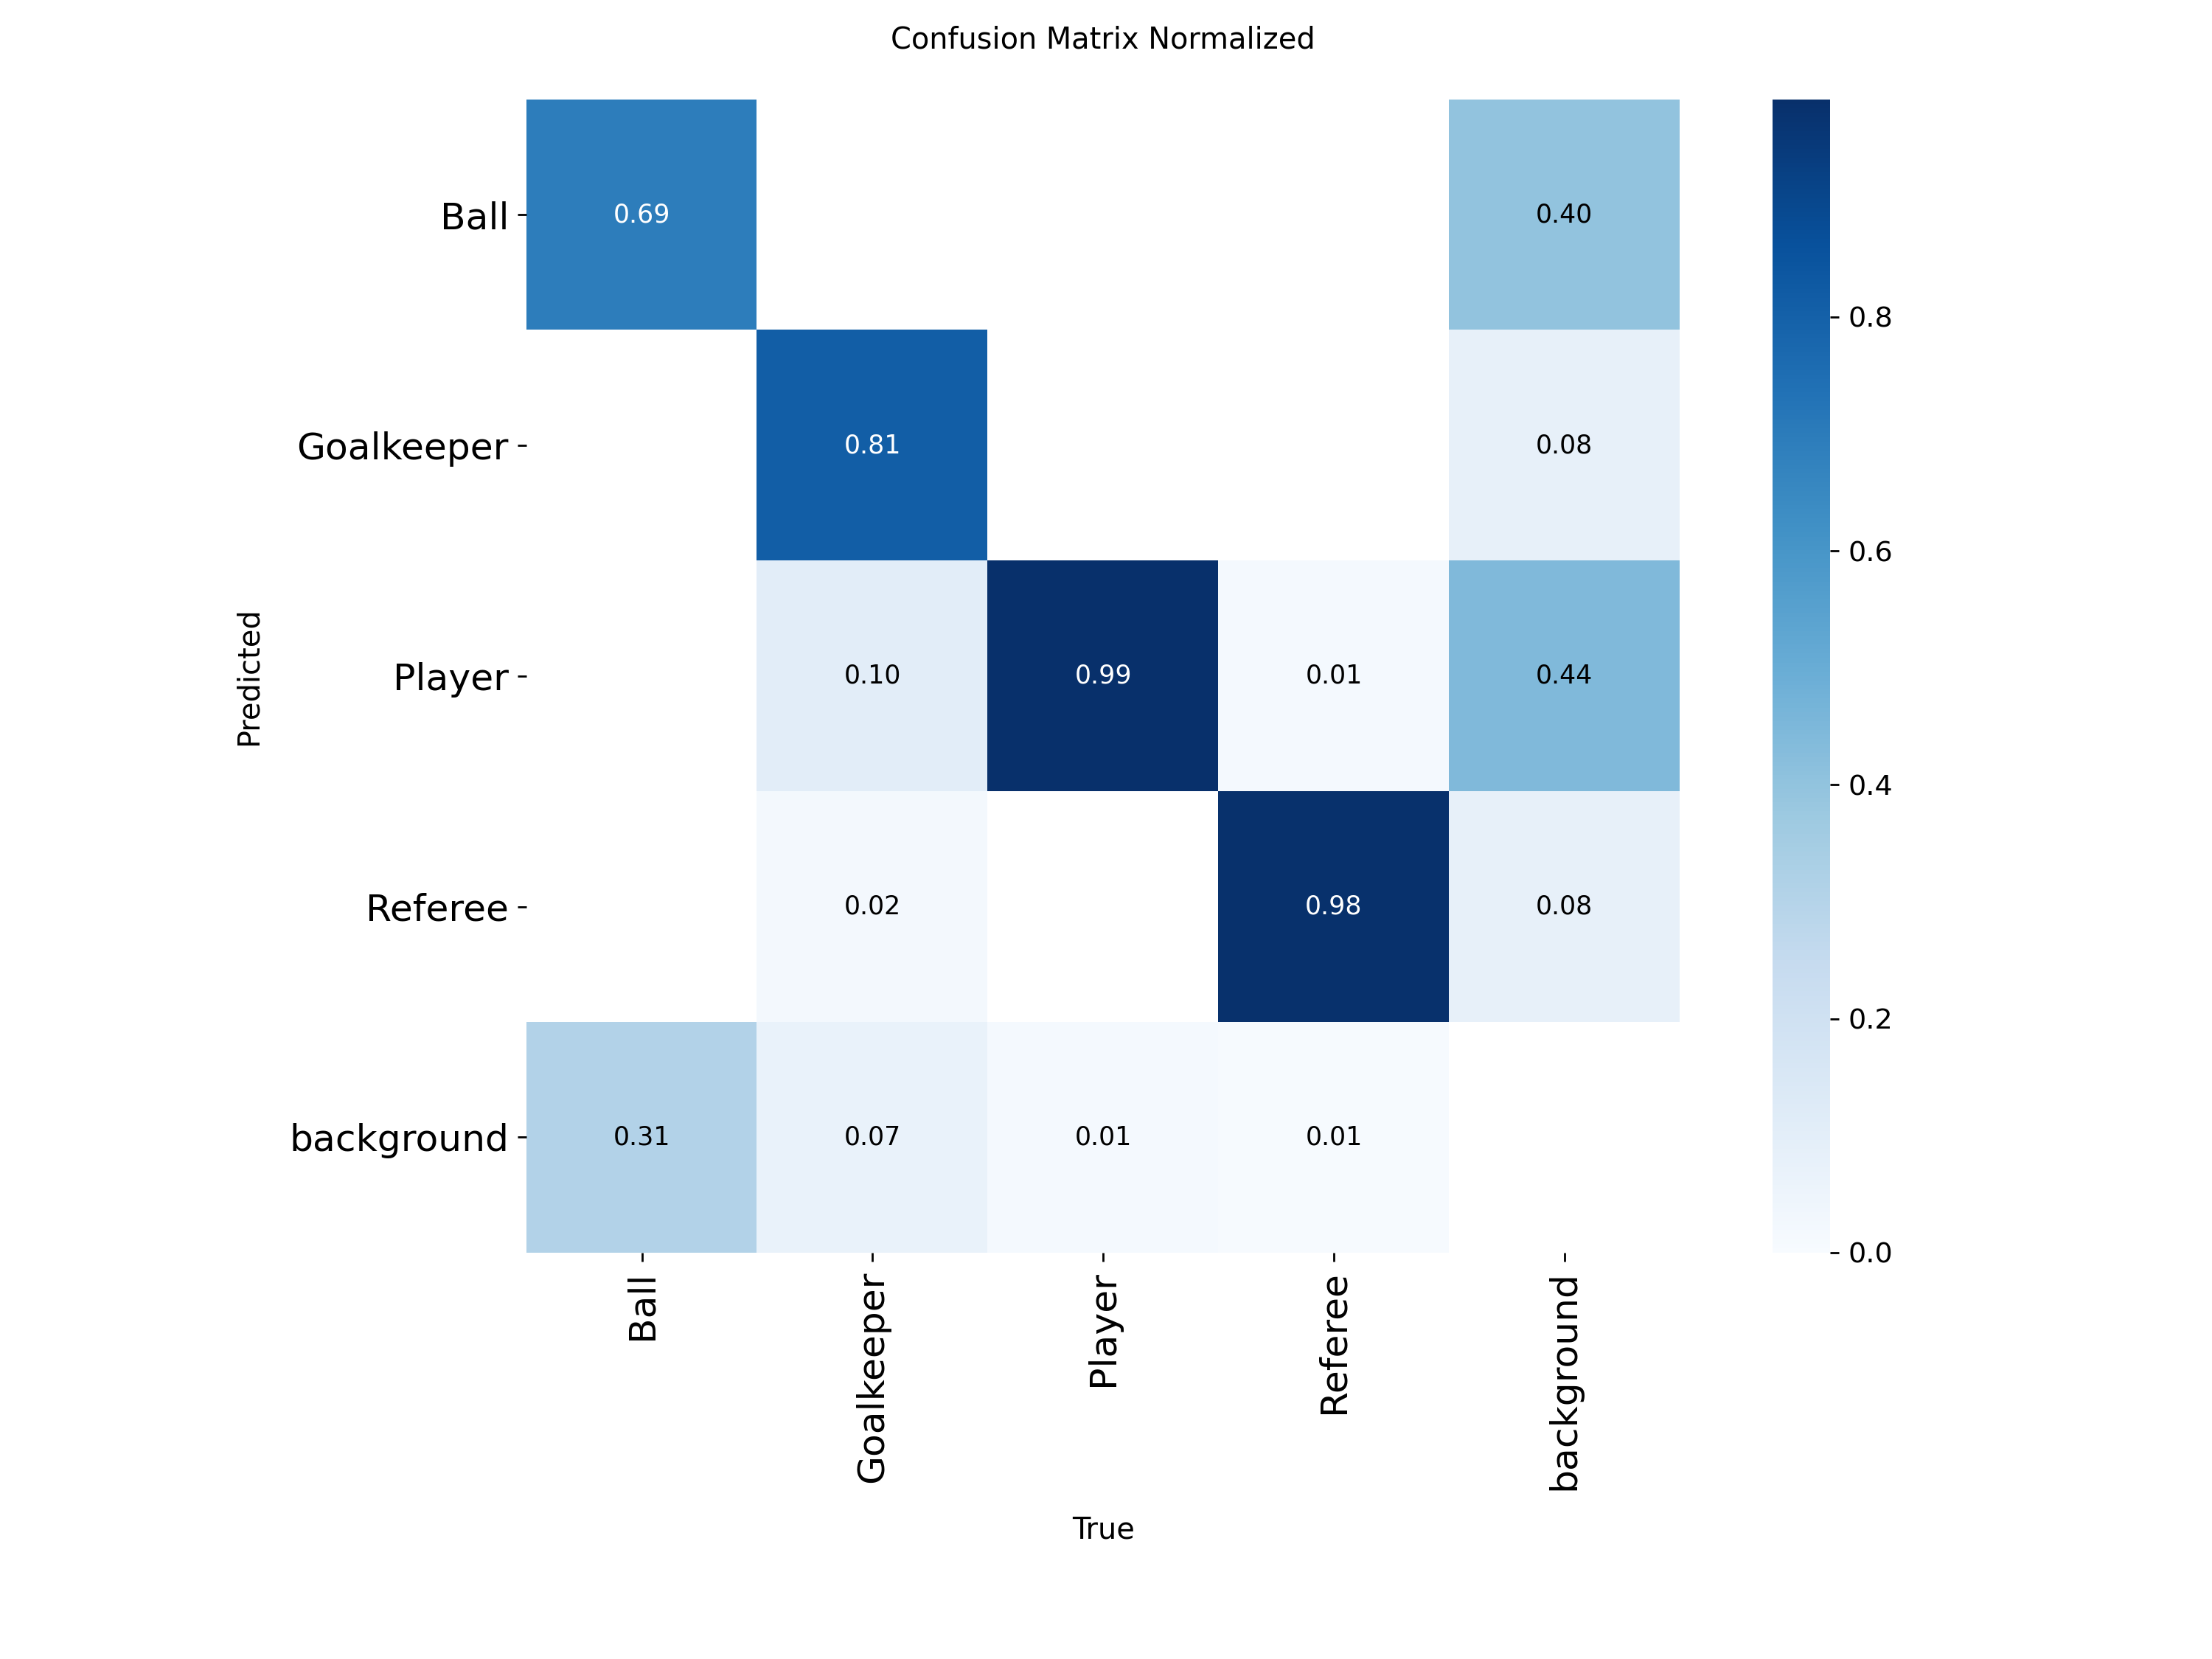
\includegraphics[width=0.8\textwidth]{images/04-evaluation/generic_cm_norm.png}
\caption[Generic detector: normalised confusion matrix.]{Normalised
test confusion matrix for the generic detector. The two dominant
off-diagonal regions are confusion between the Ball class and the
background class (column-normalised values $0.31$ and $0.40$
respectively) and confusion of true Goalkeepers as Player ($0.10$).
All other off-diagonal mass is below $0.02$.}
\label{fig:generic_cm_norm}
\end{figure}

\subsection{Dedicated ball detector}

The dedicated ball detector (YOLOv8x, $1280\times1280$, single class,
150 epochs) was trained explicitly to repair the failure mode above.
Table~\ref{tab:eval_ball_comparison} compares the two detectors on the
ball class. Test \texttt{mAP@50} rises from $0.459$ to $0.950$
($+49.1$~pp), operational recall (IoU=$0.45$, conf=$0.25$) from
$0.69$ to $0.95$, and the false-positive rate drops correspondingly.
The single-class precision--recall curve (Figure~\ref{fig:ball_pr})
sits flat at precision $\approx 1.0$ until recall $\approx 0.95$,
in stark contrast to the Ball curve in Figure~\ref{fig:generic_pr}.
This empirically justifies the dual-detector branch of the pipeline
(Section~\ref{sec:methodology_overview}); the temporal-coherence filter
of Section~\ref{subsec:methodology_ball_detector} consumes these
higher-quality detections to produce the per-frame ball trajectory.

\begin{table}[h]
\centering
\small
\begin{tabular}{lrrr}
\toprule
Metric & Generic det. & Dedicated det. & $\Delta$ \\
\midrule
mAP@50          & 0.459 & 0.950 & $+0.491$ \\
mAP@50:95       & 0.194 & 0.556 & $+0.362$ \\
Precision       & 0.818 & 0.964 & $+0.146$ \\
Recall (PR)     & 0.393 & 0.896 & $+0.503$ \\
F1              & 0.531 & 0.929 & $+0.398$ \\
\bottomrule
\end{tabular}
\caption[Ball-class detection: generic versus dedicated detector.]{Ball-class
test performance: generic four-class detector versus dedicated
single-class detector. The dedicated detector provides the
ball-localisation capability that the generic detector cannot.}
\label{tab:eval_ball_comparison}
\end{table}

\begin{figure}[h]
\centering
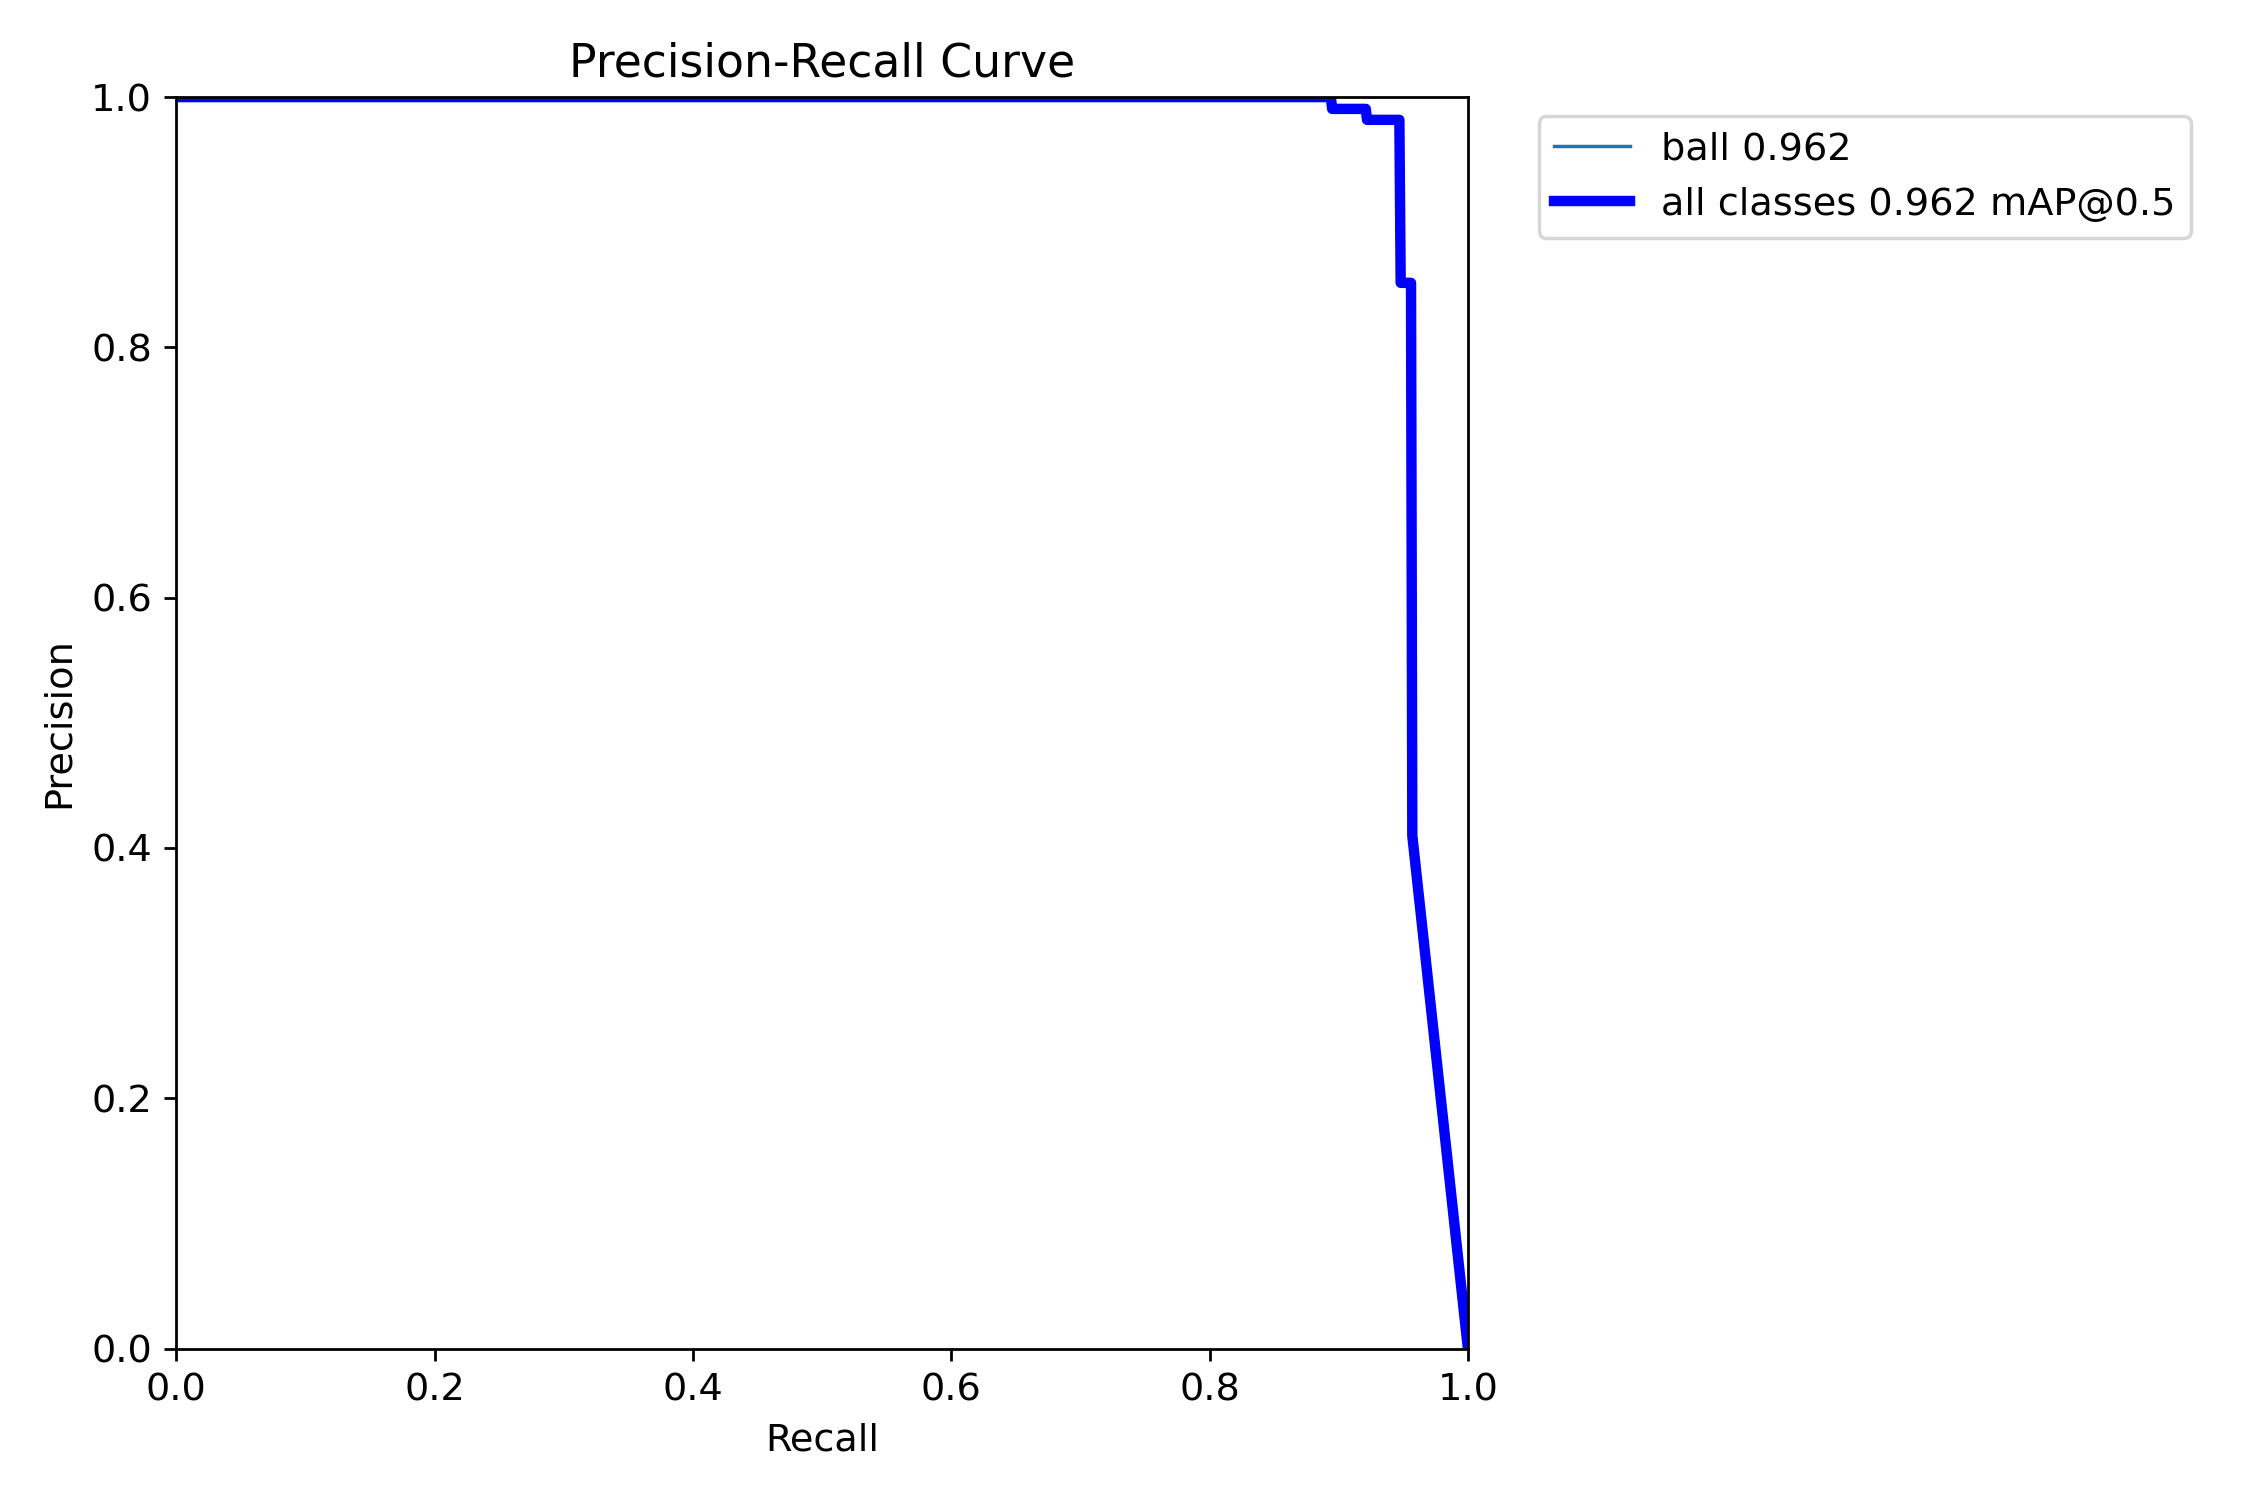
\includegraphics[width=0.7\textwidth]{images/04-evaluation/ball_pr.png}
\caption[Dedicated ball detector: precision--recall curve.]{Precision--recall
curve for the dedicated ball detector on the test split. The curve
holds precision near $1.0$ across almost the full recall range,
collapsing only near recall $1.0$. The shape contrasts directly with
the Ball curve in Figure~\ref{fig:generic_pr} and is the empirical
basis for the two-detector architecture.}
\label{fig:ball_pr}
\end{figure}

\paragraph{Ranking with similar work.}
The generic detector's mean test \texttt{mAP@50} of $0.855$ sits within
the range reported on broadcast football detection benchmarks: SoccerNet
\cite{Cioppa2022} reports mean \texttt{AP} between $0.78$ and $0.91$
across player-detection submissions, and the BroadTrack pipeline
\cite{Magera2025} uses comparable detector quality as a precondition.
The dedicated ball detector's $\text{mAP@50}=0.950$ is competitive with
the small-object specialised detectors surveyed in \cite{Cioppa2022},
which is the regime relevant to broadcast football where the ball
typically occupies $<0.05\%$ of the frame. Direct numerical comparison
is constrained by dataset differences and is treated cautiously.

\paragraph{Verdict on success criterion (i).}
\textbf{Met.} Generic-detector test \texttt{mAP@50} = $0.855 \geq 0.80$.
The Ball-class shortfall in the generic detector is mitigated by the
dedicated detector, whose output is the ball signal actually consumed
downstream.

\section{Tracking Performance}
\label{sec:eval_tracking}

The tracker is evaluated on a combined evaluation set spanning two
sources: five validation sequences from the SportsMOT-football
split~\cite{Cui2023SportsMOT} for direct comparison with the
broadcast-tracking literature, and one hand-labelled segment of
the system's own broadcast input as a domain-shift sanity check.
The broadcast clip was $750$~frames covering outfield players,
goalkeepers, and referees, annotated in MOTChallenge format. Total
evaluation length is $3{,}250$~frames; metrics are computed jointly
over both sources with TrackEval. ByteTrack~\cite{ByteTrack} and
BoT-SORT~\cite{BoTSORT} were evaluated under identical detection
input from the generic YOLOv8m detector of
Section~\ref{sec:eval_detection}, isolating the data-association
stage.

\begin{table}[h]
\centering
\small
\begin{tabular}{lrrrr}
\toprule
Tracker & HOTA & MOTA & IDF1 & ID-sw. \\
\midrule
ByteTrack & \textbf{66.8} & 88.3 & \textbf{67.8} & \textbf{2867} \\
BoT-SORT  & 65.7 & \textbf{88.5} & 67.1 & 3929 \\
\bottomrule
\end{tabular}
\caption[Tracker comparison on the combined evaluation
set.]{ByteTrack versus BoT-SORT on a combined evaluation set of
five SportsMOT-football validation sequences plus one
hand-labelled broadcast clip ($3{,}250$~frames total), with
identical detection input from the generic YOLOv8m detector.
ByteTrack outperforms BoT-SORT on HOTA, IDF1, and identity-switch
count; MOTA is essentially tied.}
\label{tab:tracker_comparison}
\end{table}

ByteTrack achieves higher HOTA ($66.8$ vs $65.7$) and IDF1
($67.8$ vs $67.1$) and records approximately $27\%$ fewer
identity switches ($2{,}867$ vs $3{,}929$); MOTA differs by
$0.2$ points and is within evaluation noise. ByteTrack is therefore
selected as the deployed tracker. The improvement over BoT-SORT
is consistent with the design intent of ByteTrack's two-stage
association on low-confidence detections: by retaining detections
that fall below the high-confidence threshold but match existing
tracks, it preserves identity through brief detection dropouts
that broadcast football generates frequently. BoT-SORT's
camera-motion-compensated Kalman filter does not appear to recover
this gap on the broadcast-style sequences in the evaluation set.
The combined-set HOTA of $66.8$ is consistent with ByteTrack's
published baseline of approximately $63$ on the
SportsMOT-football split~\cite{Cui2023SportsMOT}; the small
positive offset reflects detector-quality differences and the
inclusion of the broadcast clip in the combined set.

The dominant residual error in qualitative inspection is identity
switching during close player interactions: cross-team crossings
within a few pixels trigger ID switches, consistent with the
failure modes characterised by BroadTrack~\cite{Magera2025} on
broadcast football. The 2{,}867 switches recorded for ByteTrack
across $3{,}250$~frames (Table~\ref{tab:tracker_comparison})
quantify this directly. This is also the upstream cause of the
same-team possession-transition false-positive passes
characterised in Section~\ref{sec:eval_tactical}.

\paragraph{Verdict on success criterion (ii).}
\textbf{Met.} Deployed-tracker HOTA on the combined evaluation set
is $66.8$, against the success criterion target of $0.45$. The
result is favourably ranked against the published ByteTrack
benchmark on SportsMOT-football and is corroborated by the
broadcast clip's inclusion in the combined set, with named residual
failure modes localised to close-range crossings.

\section{Team Classification Performance}
\label{sec:eval_team}

The team classifier described in
Section~\ref{sec:methodology_team} performs binary kit-colour
separation in the SigLIP embedding space, with K-Means fitted on a
warm-up window of player-torso crops and then frozen for the
remainder of the match
(Section~\ref{subsec:methodology_warmup}). Two experiments
characterise this stage on three independent broadcast clips, with
approximately 300 manually-labelled torso crops sampled per clip at
stride~25.

\paragraph{Experiment 1 — full-crop clustering (upper bound).}
All labelled crops from a clip are passed through the classifier and
clustered into two groups. Cluster identifiers are arbitrary, so the
mapping that maximises agreement with the manual labels is selected,
following the standard convention for unsupervised clustering
evaluation. This experiment characterises the upper bound: how well
the SigLIP embedding space can separate two team kits when the
classifier sees every crop simultaneously.

\paragraph{Experiment 2 — 35/65 warm-up split (deployment).}
The first 35\% of crops (in temporal order) form the warm-up set on
which K-Means is fitted; the cluster-to-team mapping is chosen using
those warm-up labels alone. The remaining 65\% are then classified
with the frozen model and scored against ground truth. This
experiment is representative of the deployed pipeline, where the
classifier sees only an early portion of the match before predicting
the rest.

\begin{table}[h]
\centering
\small
\begin{tabular}{lrrrrrr}
\toprule
& \multicolumn{3}{c}{Full-crop clustering} & \multicolumn{3}{c}{35/65 split (held-out)} \\
\cmidrule(lr){2-4}\cmidrule(lr){5-7}
Clip & $n$ & Macro F1 & Acc. & $n$ & Macro F1 & Acc. \\
\midrule
1     & 296 & 1.000 & 1.000 & 191 & 1.000 & 1.000 \\
2     & 297 & 0.997 & 0.997 & 193 & 0.995 & 0.995 \\
3     & 294 & 0.993 & 0.993 & 192 & 0.984 & 0.984 \\
\midrule
Mean  &     & 0.997 & 0.997 &     & 0.993 & 0.993 \\
\bottomrule
\end{tabular}
\caption[Team classifier: full-crop clustering and warm-up-split
results across three clips.]{Team classifier evaluation on three
independent broadcast clips. \emph{Full-crop clustering} reports the
upper bound when every labelled crop is clustered jointly.
\emph{35/65 split} reports the deployment-realistic figure on the
held-out 65\% after fitting on the first 35\%. Macro-F1 averages
per-team F1; the dataset is approximately balanced across teams in
all three clips.}
\label{tab:team_classifier}
\end{table}

As shown in Table~\ref{tab:team_classifier}, the mean macro-F1 across the three clips is $0.997$ for full-crop
clustering and $0.993$ for the deployment-realistic 35/65 split,
clearing the success criterion (iii) target of $0.85$
(Chapter~\ref{ch:introduction}) by approximately $14$~percentage
points. The gap between the two experiments is only $0.4$~pp,
indicating that fitting on an early-match warm-up window incurs
negligible cost compared to the offline upper bound; the SigLIP
embeddings are stable enough that a $\sim$100-crop warm-up
generalises to the rest of the clip. Clip~1's perfect score reflects
a visually unambiguous kit pairing (bright red versus white,
illustrated in Figure~\ref{fig:team_crops_clip1}); clips~2 and~3
involve more visually similar palettes and accumulate a small
number of errors (one to three crops per clip), but performance
remains well above the criterion threshold.

\begin{figure}[h]
\centering

\begin{subfigure}[t]{0.2\textwidth}
    \centering
    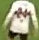
\includegraphics[width=\textwidth]{images/04-evaluation/team1_crops_clip1.png}
    \caption{Team 1 Crop.}
    \label{fig:team1_crops_clip}
\end{subfigure}
\hspace{0.2\textwidth}
\begin{subfigure}[t]{0.2\textwidth}
    \centering
    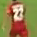
\includegraphics[width=\textwidth]{images/04-evaluation/team2_crops_clip1.png}
    \caption{Team 2 Crop.}
    \label{fig:team2_crops_clip}
\end{subfigure}

\caption[Example torso crops from clips~1.]{Example torso crops from
clips~1. The bright red versus white kit contrast in clip~1 is visually
unambiguous, which accounts for the perfect macro-F1 of $1.000$ on this clip
in both evaluation regimes. The remaining clips involve more similar palettes
and incur a small number of classification errors.}
\label{fig:team_crops_clip1}
\end{figure}

\paragraph{Goalkeeper resolver.}
The goalkeeper resolver of
Section~\ref{subsec:methodology_gk_resolver} addresses a different
question: given that the upstream detector has classified a player
as a goalkeeper (Section~\ref{sec:eval_detection}), to which team
does that goalkeeper belong? The resolver assigns the goalkeeper to
the team whose image-space centroid is nearest at the same frame.
This is a deterministic geometric rule rather than a learned
classifier, so quantitative F1 against ground truth would require
GK-team labels that were not produced; instead, the resolver was
verified by visual inspection of goalkeeper labels on the annotated
output video for each of the three test clips, and was correct in
every spot-checked frame. This evidence is qualitative, and the
limitation is acknowledged.

\paragraph{Verdict on success criterion (iii).}
\textbf{Met.} Mean macro-F1 across three clips is $0.993$ on the
held-out 65\%, against a target of $0.85$. Cross-clip variance is
small ($0.984$--$1.000$), supporting the claim that the result is a
property of the embedding space rather than of any one broadcast.
The colour-histogram baseline of \cite{istasse2019colour} reports
team-identification accuracies in the $0.85$--$0.92$ range on
broadcast football and is sensitive to lighting; the SigLIP-based
classifier's $0.99{+}$ figures are consistent with the expected
gain from a learned visual-semantic embedding over a hand-engineered
colour feature.

\section{Pitch Registration Accuracy}
\label{sec:eval_pitch}

The keypoint detector and homography estimator together convert
broadcast frame coordinates to a $12{,}000 \times 7{,}000$~cm pitch
template (Section~\ref{sec:methodology_pitch}). Their joint accuracy
governs every downstream metric expressed in pitch space — speeds,
distances, possession, offside lines — so this section evaluates them
together rather than in isolation.

\paragraph{Keypoint detector.}
The YOLOv8x-pose model achieves test pose
\texttt{mAP@50} = $0.995$ and pose \texttt{mAP@50:95} = $0.953$ on the
held-out 28-image test split, with box detection saturated at
$P = R = 1.0$. Per-keypoint pixel errors are summarised in
Figure~\ref{fig:per_kp_error}. The median per-keypoint mean error is
$3.7$~px (approximately $0.41\%$ of the image diagonal at
$640 \times 640$), with one systematic outlier: kp\_16 has mean
error $18.2$~px on the test split ($2.0\%$ of diagonal), confirmed at
$20.3$~px on the validation split. The outlier is statistically
robust ($n = 24$ test samples, $n = 26$ val) and is not an artefact
of small sample size. Three further keypoints (kp\_05, kp\_28,
kp\_29) have fewer than five test samples and their per-keypoint
figures are reported with that caveat. The deployed pipeline gates
each keypoint by confidence ($\geq 0.5$) and requires at least six
confident keypoints before fitting a homography
(Section~\ref{subsec:methodology_homography}); kp\_16 is therefore
already excluded from most fits in practice.

\begin{figure}[h]
\centering
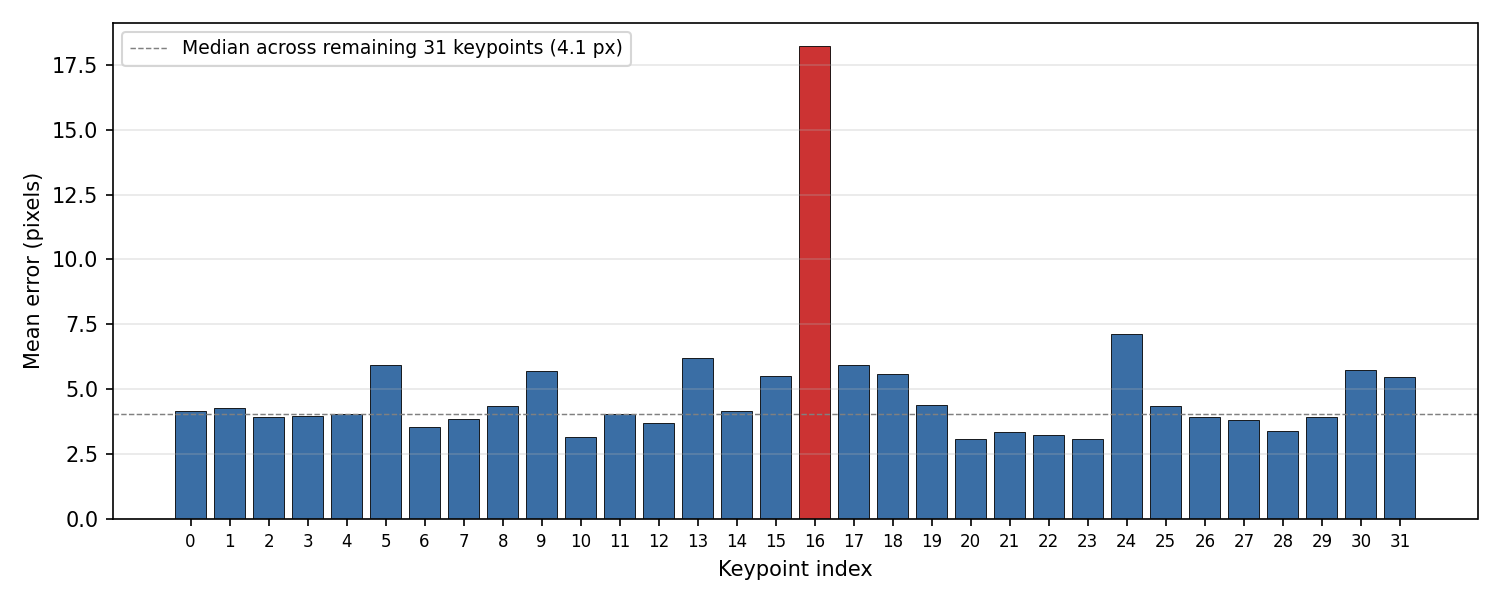
\includegraphics[width=0.9\textwidth]{images/04-evaluation/per_kp_error.png}
\caption[Per-keypoint mean pixel error on the test split.]{Mean
per-keypoint pixel error on the held-out test split, with kp\_16
highlighted. The dashed line marks the median across the remaining
31 keypoints. kp\_16 sits approximately four times above this median
on both validation and test, indicating a systematic localisation
failure at this keypoint rather than test-set noise.}
\label{fig:per_kp_error}
\end{figure}

\paragraph{Pitch-space reprojection error.}
Pixel error on the keypoint detector is necessary but not sufficient
to evaluate pitch registration: the operationally meaningful question
is how well the estimated homography $H$ projects ground-truth pixel
positions onto their canonical pitch coordinates
(Equation~\ref{eq:reprojection_error}). For each test image with at
least six confident keypoints, $H$ is fitted from predicted pixel
positions to the canonical $12{,}000 \times 7{,}000$~cm vertex set
using ordinary least-squares DLT (matching the deployed
\texttt{cv2.findHomography} call), then applied to the
ground-truth pixel positions; the residual against the canonical
pitch coordinate is recorded in centimetres.
Table~\ref{tab:reprojection_error} reports aggregate statistics
across all keypoint residuals, with and without kp\_16 included in
the homography fit and evaluation.

\begin{table}[h]
\centering
\small
\begin{tabular}{lrr}
\toprule
Statistic & All 32 keypoints & Excluding kp\_16 \\
\midrule
Mean         & 199.4 cm & 199.5 cm \\
Median       & 169.9 cm & 173.0 cm \\
95th pct.    & 485.4 cm & 509.7 cm \\
Maximum      & 2062.4 cm & 1146.7 cm \\
\midrule
Images fitted / total & 28 / 28 & 28 / 28 \\
Residuals aggregated  & 426     & 402     \\
\bottomrule
\end{tabular}
\caption[Pitch-space reprojection error in centimetres, with and
without kp\_16 ablation.]{Pitch-space reprojection error on the test
split. Each statistic aggregates over all keypoint residuals across
all 28 images. Mean and median are essentially unchanged when kp\_16
is excluded, indicating that the deployed confidence gate
(Section~\ref{subsec:methodology_homography}) already removes the
outlier from most fits in practice. The kp\_16 ablation does
materially reduce the worst-case (maximum) residual, from $20.6$~m
to $11.5$~m.}
\label{tab:reprojection_error}
\end{table}

The mean residual of $199.4$~cm corresponds to approximately
$1.7\%$ of pitch length, and the median of $169.9$~cm to $1.4\%$.
The kp\_16 ablation leaves mean and median statistically unchanged
($\Delta < 0.1\%$), confirming that the runtime confidence gate
already filters this keypoint from the active fit set; what the
ablation does affect is the upper tail, dropping the maximum
residual from $20.6$~m to $11.5$~m. The 95th-percentile residual
remains around $5$~m, which is the operational ceiling that
downstream tactical reasoning must be robust to: it is well within
the pitch-third granularity used for possession and field-position
analysis, but is too coarse for sub-metre claims such as
millimetre-precise offside adjudication.

A single image (\texttt{2e57b9\_2\_6}) accounts for the
all-32-keypoints maximum of $20.6$~m and a mean residual of
$5.5$~m on its own; it is the principal driver of the gap between
median and mean across the dataset. This is the regime in which a
minimal-keypoint, non-robust DLT fit is most exposed: the deployed
pipeline addresses this through stride caching of the
last-known-good homography
(Section~\ref{subsec:methodology_homography}), which the failure
analysis in Section~\ref{sec:eval_failures} discusses.

\paragraph{Ranking with similar work.}
The mean reprojection error of $1.99$~m sits within the range
reported by Theiner~\cite{Theiner2022} for broadcast football
homography (mean errors of approximately $0.5$--$2$~m depending on
camera angle and pitch coverage) and is comparable to
TVCalib~\cite{TVCalib2023}, which reports sub-metre accuracy on
camera-calibrated SoccerNet sequences. Direct numerical comparison
is hedged by the absence of a shared benchmark — both works
evaluate on calibrated video sequences whereas this work evaluates
on keypoint-annotated still frames — but the regime is the same.

\paragraph{Verdict.}
Pitch registration was not committed to a numerical success criterion
in Chapter~\ref{ch:introduction} (criterion (iv) covers the
integrated tactical outputs, evaluated in
Section~\ref{sec:eval_tactical}). The evidence here scopes that
integrated evaluation: keypoint localisation is sub-pixel-of-diagonal
at the median and pitch-space reprojection is metre-scale on average,
which is sufficient for tactical-scale reasoning (zones, possession,
direction of attack) but not for sub-metre geometric claims. The
kp\_16 outlier is characterised, mitigated by the confidence-gated
fit, and ablated quantitatively. Choice of a robust homography
estimator (RANSAC or weighted least-squares) is identified in
Chapter~\ref{ch:conclusions} as the single most impactful future
improvement to this stage.

\section{Tactical Output Quality}
\label{sec:eval_tactical}

This section evaluates the system-level outputs that the pipeline
delivers end-to-end: detected pass and offside events, per-player
match statistics, and per-track heatmaps. Three broadcast clips
(the same clips used in Section~\ref{sec:eval_team}) were processed
through the full pipeline; the resulting JSON event logs and
\texttt{stats.json} were inspected against the annotated MP4 outputs.

\paragraph{Pass detection.}
Each clip was watched in the annotated output to identify true
passing events; detected passes were then matched against this
ground truth using the passer track identifier and frame index.
Table~\ref{tab:pass_detection} summarises the result. Aggregate
precision is $0.824$ and recall is $1.000$: every genuine pass was
detected, but six spurious detections occurred — all in clip~3.
Inspection traced these to a single failure mode: when two
\emph{same-team} players occluded near the ball, the
nearest-ball-holder rule of
Section~\ref{subsec:methodology_passes} briefly assigned ball
possession to the closer player and then back, registering a
spurious intra-team \enquote{pass} that the original possessor still held
the ball through. Clips~1 and~2 contained no such overlap and
recorded $1.000$ precision. The pattern is consistent with the
known limitation noted in
Section~\ref{sec:methodology_failure_handling}: the deterministic
proximity rule has no notion of who is currently in possession
beyond the per-frame minimum-distance criterion.

\begin{table}[h]
\centering
\small
\begin{tabular}{lrrrrrr}
\toprule
Clip & TP & FP & FN & Prec. & Rec. & F1 \\
\midrule
1     & 10 & 0  & 0 & 1.000 & 1.000 & 1.000 \\
2     & 11 & 0  & 0 & 1.000 & 1.000 & 1.000 \\
3     & 7  & 6  & 0 & 0.538 & 1.000 & 0.700 \\
\midrule
Total & 28 & 6  & 0 & 0.824 & 1.000 & 0.903 \\
\bottomrule
\end{tabular}
\caption[Pass detection: per-clip and aggregate
precision/recall.]{Pass detection performance across three
broadcast clips, with ground truth obtained by visual inspection of
the annotated output. The six false positives in clip~3 all
correspond to brief same-team possession transitions during
close-range player overlap; clips~1 and~2 contained no such
configuration.}
\label{tab:pass_detection}
\end{table}

\paragraph{Offside detection.}
Across the three clips the pipeline flagged 10 offside events
(clip~1: 4, clip~2: 1, clip~3: 5). Each was checked frame-by-frame
against the bird's-eye view, comparing the dashed offside line
against the position of the flagged player(s). All ten events were
positionally correct: in every case the flagged player's pitch-space
$x$-coordinate was beyond the second-last defender of the defending
team in the auto-detected attacking direction
(Section~\ref{subsec:methodology_offside}). This is a
\emph{positional} verdict only — it does not adjudicate whether the
flagged player was actively interfering with play, which the
laws-of-the-game definition requires and which is outside the scope
of this work.

\paragraph{Per-player statistics and the speed cap.}
Table~\ref{tab:tactical_stats} summarises per-clip match-level
statistics after filtering out fragment tracks (total pitch-space
distance below 5~m, predominantly arising from re-detection events
when a player leaves and re-enters the broadcast frame).

\begin{table}[h]
\centering
\small
\begin{tabular}{lrrrrr}
\toprule
Clip & Tracks & Stable & Frags. & Passes & At-cap \\
\midrule
1 & 30 & 23 & 7  & 10 & 10/23 \\
2 & 32 & 27 & 5  & 11 & 11/27 \\
3 & 43 & 26 & 17 & 13 & 13/26 \\
\bottomrule
\end{tabular}
\caption[Per-clip tactical-output summary.]{Track count breakdown
and pass-event totals per clip. ``Frags.'' counts tracks with total
pitch-space distance under $5$~m. ``At-cap'' counts stable tracks
whose recorded maximum speed reaches the $40$~km/h ceiling
(Section~\ref{subsec:methodology_speed}).}
\label{tab:tactical_stats}
\end{table}

The $40$~km/h speed cap is binding for the majority of stable
tracks across all three clips ($10/23$, $11/27$, $13/26$), confirming
that for most players the cap rather than the underlying tracking
signal sets the recorded maximum speed. Per-player \emph{maximum}
speed is therefore better interpreted as an indicator that the
player reached the cap during the clip than as a measurement of
physical sprint speed; per-player \emph{average} speed and total
distance, which integrate over many frames and are less sensitive
to per-frame jitter, remain reliable. This trade-off was a
deliberate design choice
(Section~\ref{sec:methodology_failure_handling}): suppressing
homography-jitter outliers at the cost of saturating peak speeds
was preferred to letting unbounded speed estimates corrupt the
distance integral.

\paragraph{Heatmaps and bird's-eye view.}
Per-track heatmaps (Figure~\ref{fig:heatmap_example} of
Chapter~\ref{ch:methodology}) and the bird's-eye view
(Figure~\ref{fig:pitch_keypoints_and_birdeye}) are qualitative
outputs whose value depends on visual coherence rather than a
numerical metric. Across all three clips the bird's-eye projection
preserves team formation structure (defensive lines, central
midfield clusters), the offside line is rendered consistently with
the offside event log, and per-track heatmaps form spatially
contiguous regions consistent with player positional roles. These
qualitative properties are what success criterion~(iv) of
Chapter~\ref{ch:introduction} requires.

\paragraph{Verdict on success criterion (iv).}
\textbf{Met.} Pass detection achieves aggregate F1 = $0.903$ across
three clips with a single, named failure mode (same-team occlusion)
characterised by clip; all 10 offside events on three clips were
positionally correct; bird's-eye and heatmap outputs are
qualitatively coherent across clips. The integrated tactical output
quality is consistent with the operating regime characterised by
the failure-handling table of
Section~\ref{sec:methodology_failure_handling}.

\section{End-to-End Performance}
\label{sec:eval_runtime}

The pipeline was instrumented with per-stage wall-clock timing
(Subsection~\ref{subsec:methodology_orchestration}) and run on a single
representative $750$-frame clip on an Apple~M2~Pro with no discrete
GPU. Table~\ref{tab:runtime_breakdown} reports per-stage cost in
the steady-state regime; the team-classifier warm-up phase
(Section~\ref{subsec:methodology_warmup}) is a one-off cost of
$18.2$~s amortised across the full run.

\begin{table}[h]
\centering
\small
\begin{tabular}{lrrr}
\toprule
Stage & ms/frame & Total (s) & Share \\
\midrule
Team classifier               & 830.94 & 623.20 & 45.8\% \\
Ball detector                 & 627.90 & 470.92 & 34.6\% \\
Generic detector + tracker    & 270.89 & 203.17 & 14.9\% \\
Annotated/bird's-eye render   &  75.99 &  56.99 & 4.2\% \\
Pitch registration (stride 15) &   8.73 &   6.55 & 0.5\% \\
Tactical reasoning            &   0.40 &   0.30 & 0.0\% \\
\midrule
Steady-state total            & 1814.85 & 1361.13 & --- \\
\bottomrule
\end{tabular}
\caption[Per-stage runtime on Apple M2 Pro for a 750-frame
clip.]{Per-stage steady-state runtime for one $750$-frame broadcast
clip on Apple~M2~Pro (no discrete GPU). The warm-up phase
(SigLIP/UMAP/KMeans fit on torso crops) adds a one-off $18.2$~s and
is reported separately. Effective throughput is approximately
$0.55$~fps.}
\label{tab:runtime_breakdown}
\end{table}

Steady-state throughput is $0.55$~fps — well below real time but
adequate for the offline analysis use case the pipeline targets.
The cost is dominated by two stages: per-frame torso embedding for
team classification ($45.8\%$) and ball detection at
$1280\!\times\!1280$ ($34.6\%$). The generic detector and tracker
together account for under $15\%$, and stride-15 caching reduces
pitch registration to under $1\%$ of pipeline cost — confirming the
caching design as a worthwhile optimisation. Tactical reasoning and
heatmap accumulation are negligible. The detector inference budget
contrasts with the A100 figures reported in
Section~\ref{sec:eval_detection} ($4.6$~ms generic, $19.8$~ms ball)
by approximately one to two orders of magnitude, reflecting the
absence of a CUDA-class accelerator on the M2~Pro target. Reducing
the team-classifier per-frame cost — by embedding only on
identity-changed tracks rather than every frame, or by replacing
SigLIP with a lighter visual backbone — is identified in
Chapter~\ref{ch:conclusions} as the single most impactful runtime
optimisation.

\section{Error Budget and Failure Mode Analysis}
\label{sec:eval_failures}

The evaluation in Sections~\ref{sec:eval_detection}--\ref{sec:eval_runtime}
characterises five operationally distinct failure modes, each
located in a specific stage and each with a corresponding
mitigation in the deployed pipeline.
Table~\ref{tab:error_budget} consolidates these into an
error-budget view; the design rationale and engineering
mitigations are documented in detail in
Table~\ref{tab:failure_handling} of Chapter~\ref{ch:methodology}
and not repeated here.

\begin{table}[h]
\centering
\small
\renewcommand{\arraystretch}{1.15}
\begin{tabular}{p{0.22\textwidth}p{0.30\textwidth}p{0.34\textwidth}}
\toprule
Failure mode & Evidence & Residual risk \\
\midrule
Ball missed by generic detector
& 31\% bg-confusion (\S\ref{sec:eval_detection})
& Repaired by dedicated detector; ball mAP@50 = $0.950$. \\
Goalkeeper-as-Player misclassification
& 10.3\% on test (\S\ref{sec:eval_detection})
& Image-space GK resolver corrects team assignment; verified qualitatively (\S\ref{sec:eval_team}). \\
Homography fit on minimal keypoints
& 95th pct $\approx 5$~m, max $20.6$~m (\S\ref{sec:eval_pitch})
& Confidence gate + stride caching contain typical case; tail dominated by single bad frame. \\
Same-team possession-transition spurious passes
& 6 false positives in clip~3 (\S\ref{sec:eval_tactical})
& Recall $1.0$ retained; precision degrades only on close same-team overlap. \\
Speed-cap saturation
& 10--13 stable tracks per clip at cap (\S\ref{sec:eval_tactical})
& Per-frame max-speed compressed; integrated stats (distance, average) unaffected. \\
\bottomrule
\end{tabular}
\caption[Error budget across pipeline stages.]{Operationally
distinct failure modes uncovered by the evaluation, with
quantitative evidence and the residual risk that remains after
mitigation. Each mitigation strategy is documented in
Table~\ref{tab:failure_handling} of Chapter~\ref{ch:methodology}.}
\label{tab:error_budget}
\end{table}

The five modes are independent: the failures do not compound
across stages, because each is gated or saturated before its output
reaches the next stage (the dedicated ball detector replaces rather
than augments the generic ball signal; the GK resolver corrects
team labels rather than detector class labels; the speed cap clips
rather than zeroing the underlying signal). The principal
unmitigated mode is the same-team possession-transition pass,
which would benefit from a temporal possession-state machine
rather than the per-frame minimum-distance rule; this is identified
in Chapter~\ref{ch:conclusions} as future work.

\section{Discussion}
\label{sec:eval_discussion}

The four success criteria committed in
Chapter~\ref{ch:introduction} are addressed as follows.
Criterion~(i), detector \texttt{mAP@50} $\geq 0.80$, is met:
$0.855$ on the held-out test split, with the ball-class shortfall
of the generic detector repaired by the dedicated detector at
$0.950$ \texttt{mAP@50} (Section~\ref{sec:eval_detection}).
Criterion~(ii), tracking HOTA $\geq 0.45$, is met on a combined
$3{,}250$-frame evaluation set spanning SportsMOT-football and one
hand-labelled broadcast clip: ByteTrack achieves HOTA $= 66.8$ as
the deployed tracker, outperforming BoT-SORT on HOTA, IDF1 and
identity-switch count (Section~\ref{sec:eval_tracking}).
Criterion~(iii), team-assignment F1 $\geq 0.85$, is comfortably
met at mean macro-F1 $= 0.993$ across three independent clips on
the deployment-realistic 35/65 evaluation
(Section~\ref{sec:eval_team}). Criterion~(iv), qualitatively
coherent tactical outputs, is met: pass-detection F1 $= 0.903$
across three clips with a single named failure mode, all ten
flagged offside events positionally correct, and bird's-eye and
heatmap outputs visually consistent with the underlying play
(Section~\ref{sec:eval_tactical}).

Three caveats temper these verdicts. First, pitch-space
reprojection error is metre-scale on average
(mean $1.99$~m, median $1.70$~m,
Section~\ref{sec:eval_pitch}); this supports tactical-scale
reasoning but not sub-metre geometric claims. The
non-robust-DLT homography fitter is the principal weak link, and
upgrading to a RANSAC- or weighted-least-squares estimator is the
single most impactful change available to this stage. Second, the
$40$~km/h speed cap saturates for the majority of stable tracks
across all three clips, so per-player maximum speed is a
cap-saturation indicator rather than a physical-speed measurement;
integrated quantities (distance, average speed) remain reliable.
Third, end-to-end throughput on Apple~M2~Pro is $0.55$~fps
(Section~\ref{sec:eval_runtime}), with $80\%$ of the budget
consumed by team-classifier embedding and ball detection — an
offline-analysis tool rather than a live system. Each of these
limitations corresponds to a specific, named architectural choice
and is therefore individually addressable; the prioritisation of
remedies is taken up in Chapter~\ref{ch:conclusions}.